\documentclass[]{article}
\usepackage[UTF8]{ctex}
\usepackage{float}
\usepackage{amsmath}
\usepackage{url}
\usepackage{graphicx}
\usepackage{algorithm} 
\usepackage{xcolor}
\usepackage{algpseudocode}  
\usepackage{booktabs}
\usepackage{listings}
\usepackage{hyperref}

%opening
\title{NNDL课后作业}
\author{盛焕新15220202202189}

\begin{document}

\maketitle


\section{第二章课后习题}
\begin{figure}[H]
	\centering
	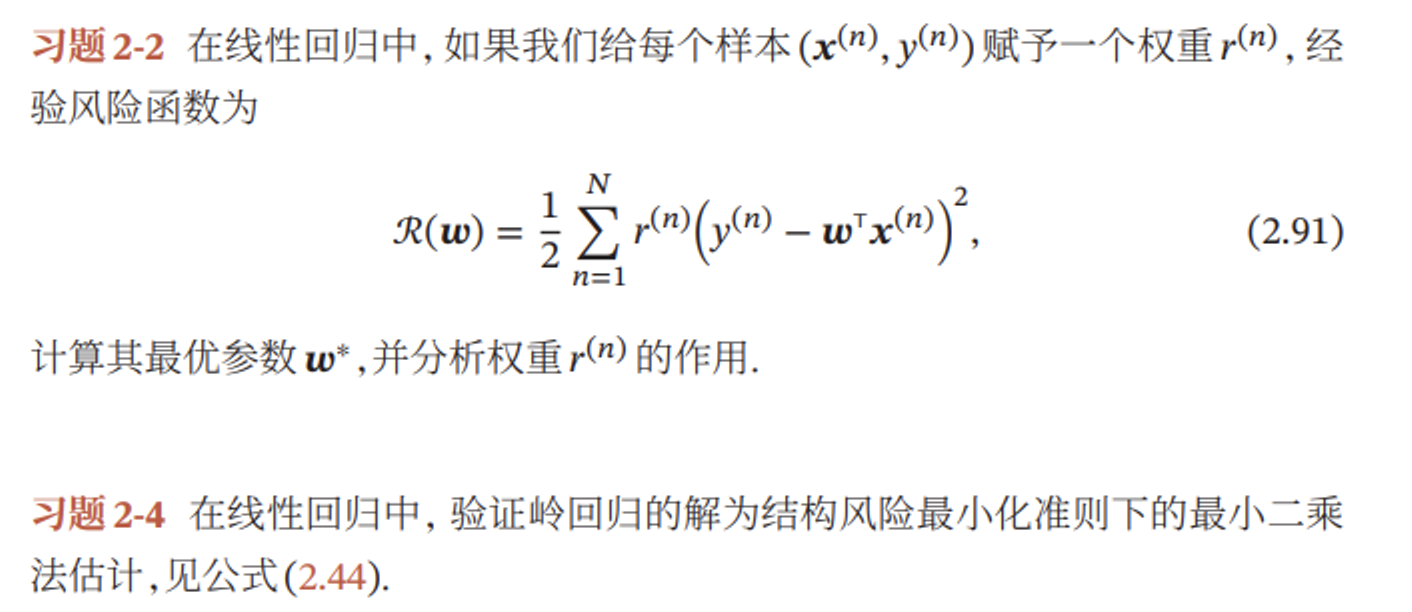
\includegraphics[width=1\linewidth]{第二章课后习题}
	\caption{第二章课后习题}
	\label{fig:}
\end{figure}
\subsection{习题2-2}
首先,我们计算经验风险函数 $\mathcal{R}(\boldsymbol{w})$ 的梯度:
$$
\frac{\partial \mathcal{R}(\boldsymbol{w})}{\partial \boldsymbol{w}} = - \sum_{n=1}^N r^{(n)} \left( \mathbf{y}^{(n)} - \boldsymbol{w}^{\top} \mathbf{x}^{(n)} \right) \mathbf{x}^{(n)^{\top}}.
$$

然后,我们令该梯度等于零,解得最优参数 $\boldsymbol{w}^*$:
$$
\frac{\partial \mathcal{R}(\boldsymbol{w})}{\partial \boldsymbol{w}} = 0 \Rightarrow \sum_{n=1}^N r^{(n)} \left( y^{(n)} - \mathbf{w}^{\top} \mathbf{x}^{(n)} \right) \mathbf{x}^{(n)^{\top}} = 0.
$$

解得:
$$
\mathbf{w}^* = \left( \sum_{n=1}^N r^{(n)} \mathbf{x}^{(n)} \mathbf{x}^{(n)^{\top}} \right)^{-1} \left( \sum_{n=1}^N r^{(n)} y^{(n)} \mathbf{x}^{(n)^{\top}} \right).
$$

接下来,我们分析权重 $r^{(n)}$ 的作用。当 $r^{(n)} = 1$ 时,权重 $r^{(n)}$ 对经验风险函数没有影响,此时 $\mathbf{w}^*$ 退化为最小二乘法的解。

当 $r^{(n)} > 1$ 时,权重 $r^{(n)}$ 会增加相应样本的权重,使得该样本在计算最优参数时具有更大的影响力。

当 $r^{(n)} < 1$ 时,权重 $r^{(n)}$ 会减小相应样本的权重,使得该样本在计算最优参数时的影响力减小。

因此,通过调整权重 $r^{(n)}$,我们可以对不同样本在计算最优参数时的权重进行调整,从而更好地拟合数据。这个方法叫做加权最小二乘(如果我没记错的话)。它的想法就是,因为不同的样本对模型的影响不同,我们希望对不同的样本给予不同的权重以便得到更高的模型准确率。


\subsection{习题2-4}

首先,我们定义结构风险函数为:
$$
J(\mathbf{w}) = \frac{1}{2} \sum_{n=1}^N r^{(n)} \left( y^{(n)} - \mathbf{w}^{\top} \mathbf{x}^{(n)^{\top}} \right)^2 + \lambda \|\mathbf{w}\|^2,
$$
其中 $\lambda$ 是岭回归的正则化参数,用于控制模型复杂度,它能够克服数据中的多重共线性的问题。梯度求解令为0,即可解得岭回归的解:
$$
\frac{\partial J(\mathbf{w})}{\partial \mathbf{w}} = 0 \Rightarrow \sum_{n=1}^N r^{(n)} \left( y^{(n)} - \mathbf{w}^{\top} \mathbf{x}^{(n)} \right) \mathbf{x}^{(n)^{\top}} + 2\lambda \mathbf{w} = 0.
$$

解得:
$$
\mathbf{w}^* = \left( \sum_{n=1}^N r^{(n)} \mathbf{x}^{(n)} \mathbf{x}^{(n)^{\top}} - 2\lambda I \right)^{-1} \left( \sum_{n=1}^N r^{(n)} y^{(n)} \mathbf{x}^{(n)^{\top}} \right).
$$

最后,我们观察解 $\mathbf{w}^*$,可以看出它实际上是结构风险函数的最小化解。因此,岭回归的解满足结构风险最小化准则下的最小二乘法估计。


\section{第三章课后习题}
\begin{figure}[H]
	\centering
	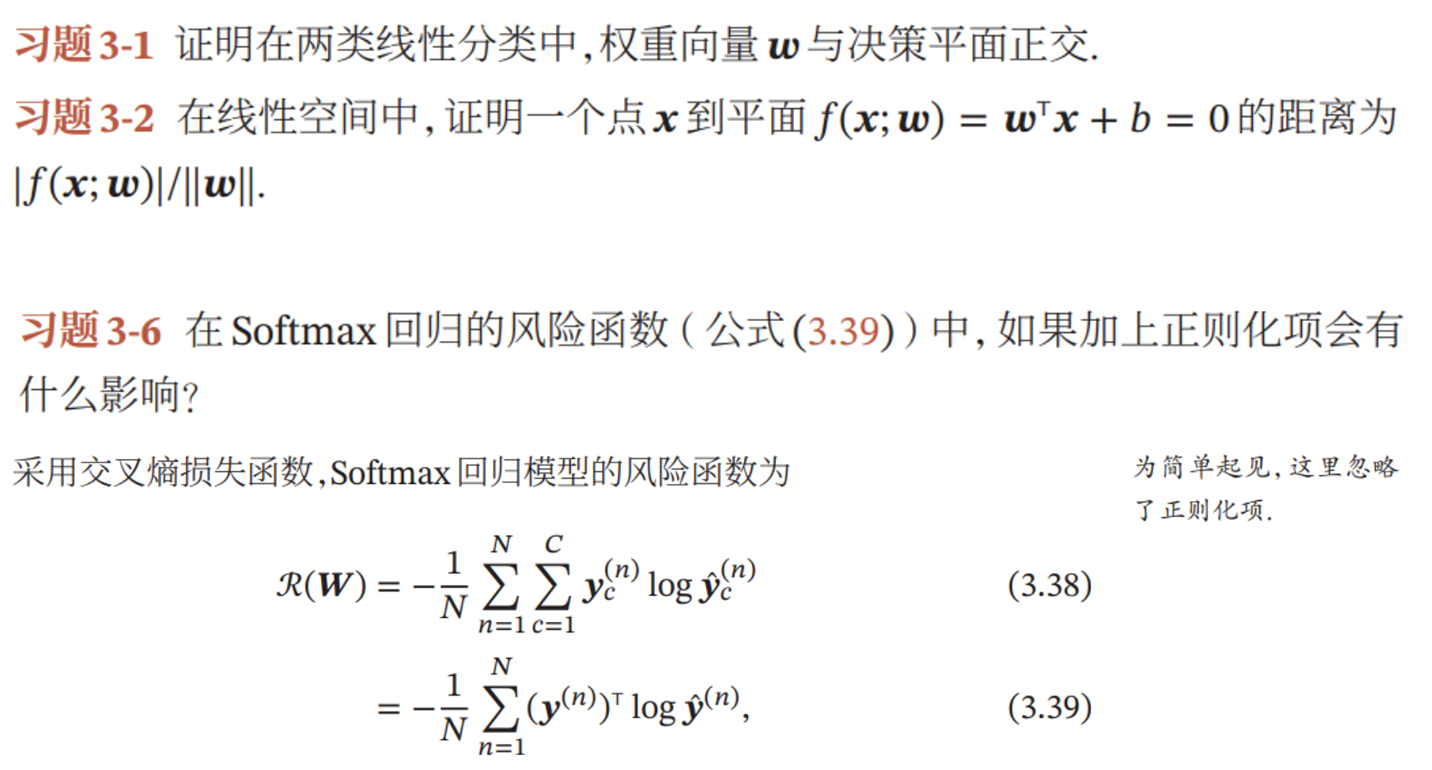
\includegraphics[width=1\linewidth]{第三章课后习题}
	\caption{第三章课后习题}
	\label{fig:}
\end{figure}
\subsection{习题3-1}
首先,根据线性分类的定义,我们知道决策函数 $f(x) = \mathbf{w}^{\top} \mathbf{x}$ 的输出值决定了样本点 $\mathbf{x}$ 属于哪一类。

然后,根据线性分类的几何解释,决策平面是 $\mathbf{w}^{\top} \mathbf{x} = 0$,而权重向量 $\mathbf{w}$ 垂直于这个平面。

接着,根据向量正交的定义,两个向量正交当且仅当它们的点积为零。由于决策平面与权重向量 $\mathbf{w}$ 正交,所以 $\mathbf{w}^{\top} \mathbf{x}$ 与 $\mathbf{w}$ 也正交。所以 $\mathbf{w}^{\top} \mathbf{w} = 0$。

综上,我们证明了在两类线性分类中,权重向量 $\mathbf{w}$ 与决策平面正交。
\subsection{习题3-2}
首先,根据点到平面的距离公式,点 $\mathbf{x}$ 到平面 $Ax + By + Cz + D = 0$ 的距离为 $\frac{|Ax + By + Cz + D|}{\sqrt{A^2 + B^2 + C^2}}$。我们可以将平面 $f(\mathbf{x} ; \mathbf{w}) = \mathbf{w}^{\top} \mathbf{x} + b = 0$ 写成标准形式,即 $w_1 x_1 + w_2 x_2 + \ldots + w_n x_n + b = 0$。然后代入公式,就可以得到点 $\mathbf{x}$ 到平面 $f(\mathbf{x} ; \mathbf{w}) = 0$ 的距离为:
$$\frac{|w_1 x_1 + w_2 x_2 + \ldots + w_n x_n + b|}{\sqrt{w_1^2 + w_2^2 + \ldots + w_n^2}} =\frac{|\mathbf{w}^{\top} \mathbf{x} + b|}{\|\mathbf{w}\|} =  \frac{|f(\mathbf{x} ; \mathbf{w})|}{\|\mathbf{w}\|}$$.

\subsection{习题3-6}
在Softmax回归中,加上正则化项会对模型产生以下影响:

1. 防止过拟合:正则化项可以防止模型过拟合训练数据,提高模型的泛化能力。过拟合是指模型在训练数据上表现很好,但在测试数据上表现较差的现象。通过引入正则化项,可以对模型的复杂度进行约束,避免模型过于复杂而出现过拟合的情况。

2. 权重衰减:正则化项通常会对模型的权重参数进行惩罚,使得权重参数的值趋向于零。这种权重衰减的效果可以使得模型更加平滑,减少模型对训练数据中的噪声的敏感性。

3. 特征选择:正则化项还可以起到特征选择的作用。在正则化过程中,一些对模型预测结果影响较小的特征对应的权重参数会被压缩为零,从而实现特征的选择和降维。

具体来说,如果在Softmax回归的风险函数中加入L2正则化项,即权重衰减项,风险函数变为:
$$
\begin{aligned}
	\mathcal{R}(\boldsymbol{W}) & =-\frac{1}{N} \sum_{n=1}^N \sum_{c=1}^C y_{\mathrm{c}}^{(n)} \log \hat{\boldsymbol{y}}_{\mathrm{c}}^{(n)} + \frac{\lambda}{2} \|\boldsymbol{W}\|_2^2 \\
	& =-\frac{1}{N} \sum_{n=1}^N\left(\boldsymbol{y}^{(n)}\right)^{\top} \log \hat{\boldsymbol{y}}^{(n)} + \frac{\lambda}{2} \sum_{i=1}^D w_i^2,
\end{aligned}
$$
其中$\lambda > 0$是正则化系数,$D$是特征的维度,$w_i$是权重参数。通过最小化带有正则化项的风险函数,可以实现对权重参数的约束和惩罚,从而得到更加鲁棒的模型。
\section{第四章课后习题}
\begin{figure}[H]
	\centering
	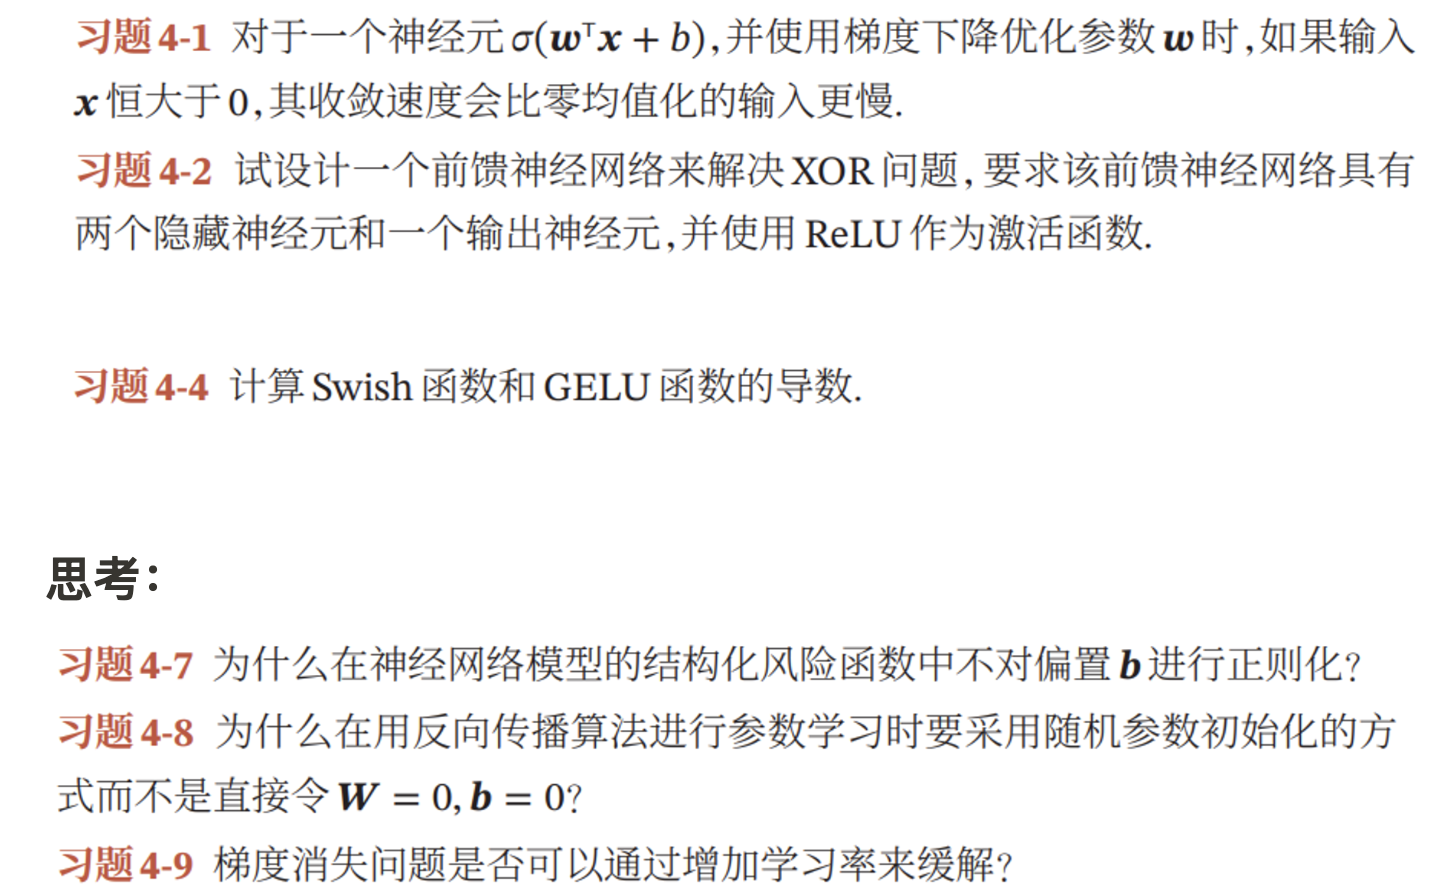
\includegraphics[width=1\linewidth]{第四章课后习题}
	\caption{第四章课后习题}
	\label{fig:}
\end{figure}

\subsection{习题4-1}
如果输入$\boldsymbol{x}$不是零均值化的,而是恒大于0的,梯度下降可能会受到输入的尺度影响,导致参数的更新步长不一致,从而降低了收敛速度。

\subsection{习题4-2}
解决 XOR 问题的前馈神经网络可以设计如下,其中包含两个隐藏神经元和一个输出神经元,激活函数选择ReLU:

Input Layer: 2 neurons (corresponding to XOR input features)

Hidden Layer: 2 neurons (using ReLU activation)

Output Layer: 1 neuron (using ReLU activation)
\subsection{习题4-4}

Swish函数:
$$Swish(x) = \frac{x}{1 + e^{-x}}$$

Swish函数的导数:
$$Swish'(x) = (1 + e^{-x})^{-2} \times e^{-x} \times (1 - x)$$

GELU函数:
$$GELU(x) = 0.5 \times x \times (1 + \tanh(\sqrt{\frac{2}{\pi}} \times (x + 0.044715 \times x^3)))$$

GELU函数的导数:
$$GELU'(x) = 0.5 \times (1 + \tanh(\sqrt{\frac{2}{\pi}} \times (x + 0.044715 \times x^3))) + 0.5 \times x \times \sqrt{\frac{2}{\pi}} \times (1 - \tanh^2(\sqrt{\frac{2}{\pi}} \times (x + 0.044715 \times x^3))) \times (2 \times 0.044715 \times x^2)$$

\subsection{习题4-7}
在神经网络模型的结构化风险函数中,通常不对偏置 \(\boldsymbol{b}\) 进行正则化的主要原因是:正则化的目的是减小模型的复杂度,防止过拟合,并提高其在未见过的数据上的泛化能力。但是,对偏置进行正则化可能导致模型无法很好地学习数据的平移。偏置通常不会引起过拟合的问题,因此在结构化风险函数中通常不对偏置进行正则化,以确保模型能够更好地适应数据的平移。

\subsection{习题4-8}
在神经网络中,采用随机参数初始化而不是将权重矩阵 \(\boldsymbol{W}\) 和偏置向量 \(\boldsymbol{b}\) 设置为零的主要是因为,设置为0时可能会导致对称性破缺和梯度消失的问题。

1. 对称性破缺:
如果将所有的权重初始化为相同的值,比如零,那么在每一次更新时,所有神经元的权重都会被同时更新,导致它们保持对称性。这就意味着无论多少层网络,每一层的神经元都在学习相同的表示,限制了网络的表达能力。通过随机初始化,我们打破了这种对称性,使得每个神经元可以学习不同的特征,提高了网络的表达能力。

2. 梯度消失问题:
如果所有权重都初始化为零,那么在反向传播算法中,由于所有神经元的梯度都相同,它们在更新时将始终保持相同的权重。这可能导致在网络较深时梯度消失或梯度爆炸的问题。通过采用随机初始化,我们引入了足够的随机性,以使得网络中的神经元在训练过程中可以学习到不同的特征,减轻了梯度消失问题。

因此,为了打破对称性、提高网络的表达能力以及防止梯度消失问题,通常采用随机参数初始化的方式,其中权重和偏置的初始值是从某个分布(例如高斯分布或均匀分布)中随机抽取的。这样可以帮助网络更好地学习数据的特征。

\subsection{习题4-9}
增加学习率并不总是有效地缓解梯度消失问题。梯度消失问题通常是由于深度神经网络中的反向传播过程中,梯度逐层相乘导致梯度变得非常小而接近零。在这种情况下,增加学习率可能会使问题更加严重,因为梯度更新的步长增大,导致权重更新过大,甚至可能发生梯度爆炸。

梯度消失问题的主要原因之一是深层网络中的激活函数具有饱和性质,如sigmoid或tanh函数。这些函数在输入较大或较小时梯度接近零,导致梯度无法有效地传递到较早层。

\section{第五章课后习题}

\begin{figure}[H]
	\centering
	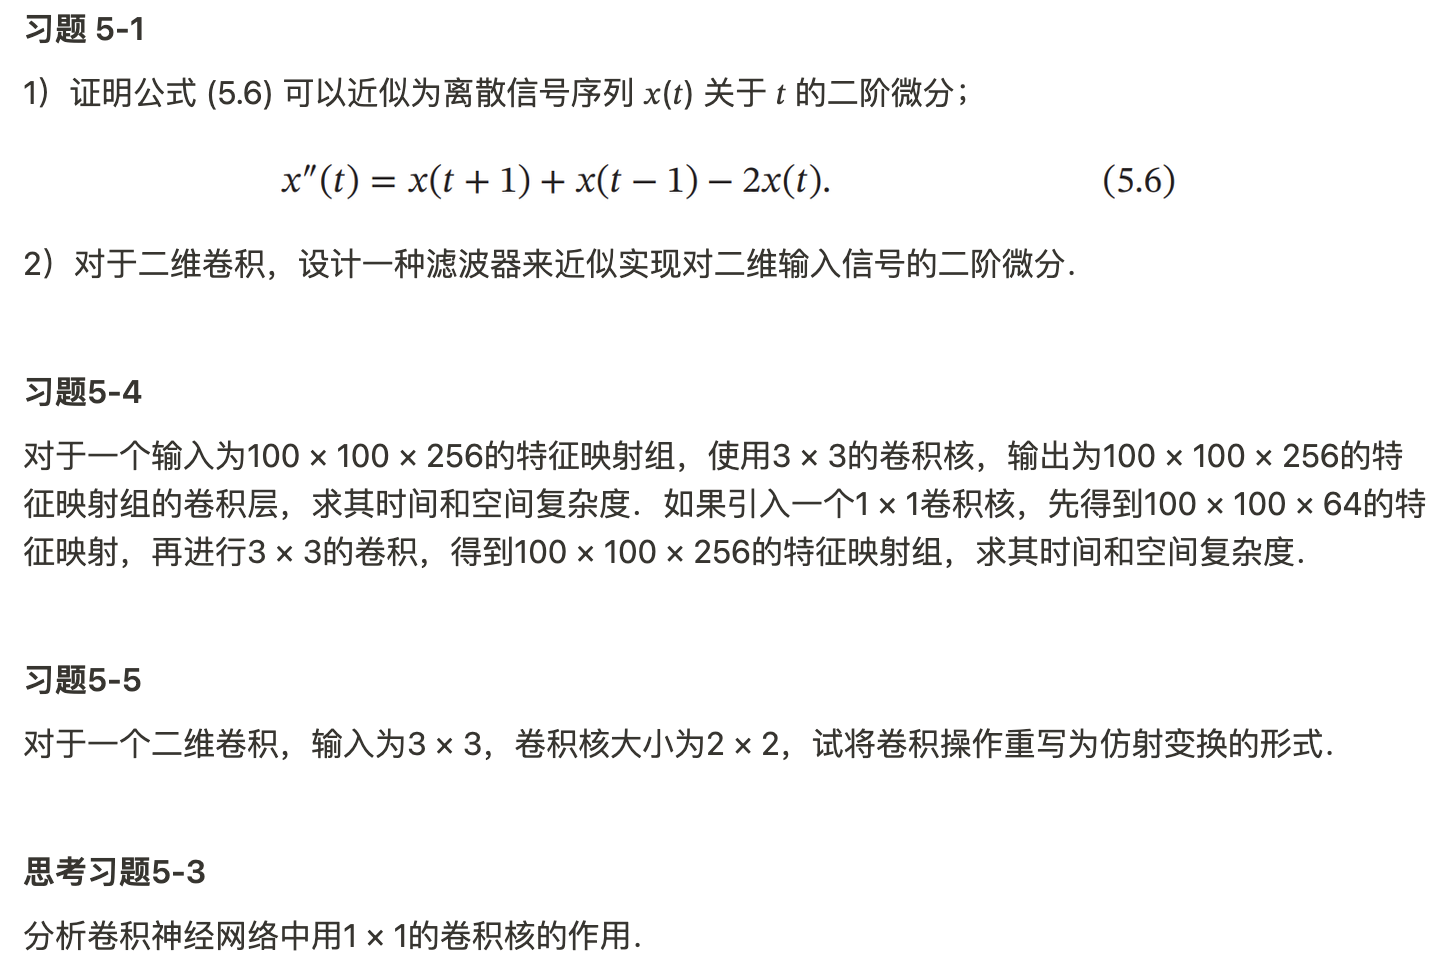
\includegraphics[width=1\linewidth]{第五章课后习题}
	\caption{第五章课后习题}
	\label{fig:}
\end{figure}

\subsection{习题5-1}
1) 证明公式 (5.6) 可以近似为离散信号序列 \(x(t)\) 关于 \(t\) 的二阶微分:
\[ x^{\prime \prime}(t) = x(t+1) + x(t-1) - 2x(t) \]

证明:

对于连续信号 \(x(t)\),它的二阶导数为
\[ x^{\prime \prime}(t) = \frac{d^2x}{dt^2} \]

我们可以使用中心差分来近似二阶导数:
\[ \frac{d^2x}{dt^2} \approx \frac{x(t+1) - 2x(t) + x(t-1)}{(\Delta t)^2} \]

这里 \(\Delta t\) 是时间步长。现在,我们将 \(t\) 替换为 \(n\)(离散时间点),并设 \(\Delta t = 1\),得到:
\[ x^{\prime \prime}(n) \approx x(n+1) + x(n-1) - 2x(n) \]

这与公式 (5.6) 是一致的,因此公式 (5.6) 可以近似为离散信号序列 \(x(t)\) 关于 \(t\) 的二阶微分。


2) 对于二维卷积,设计一种滤波器来近似实现对二维输入信号的二阶微分:

在二维卷积中,我们可以使用一个滤波器来近似实现对二维输入信号的二阶微分。一个常用的滤波器是:
\[ 
\begin{bmatrix}
	1 & -2 & 1 \\
\end{bmatrix}
\]

该滤波器对二维输入信号进行卷积操作,可以近似实现对信号在水平方向的二阶微分。这个滤波器的卷积操作可以表示为:
\[ y(m, n) = x(m, n+1) - 2x(m, n) + x(m, n-1) \]

其中,\(x(m, n)\) 是输入信号的二维数组,\(y(m, n)\) 是卷积结果。

请注意,如果要对垂直方向进行二阶微分,可以使用类似的滤波器,只是在行的方向上进行卷积。


\subsection{习题5-4}
时间复杂度:

1. 卷积操作的计算量:对于一个2D卷积操作,计算量与卷积核的大小、输入数据的大小以及通道数有关。如果卷积核的大小是 \(k \times k\),输入数据的大小是 \(n \times n\),通道数是 \(c\),那么计算量大约为 \(O(k^2 \times n^2 \times c)\)。

2. 步幅(stride):步幅是指卷积核在输入数据上滑动的步长。如果步幅是 \(s\),那么计算量将减少为 \(O\left(\frac{k^2 \times n^2 \times c}{s^2}\right)\)。

3. 多通道卷积:如果有多个输入通道,需要对每个通道进行卷积,然后将结果相加。对于 \(c\) 个输入通道,计算量将增加为 \(O(c \times k^2 \times n^2)\)。

空间复杂度:

1. 卷积核的存储:卷积核的大小决定了存储空间的需求。存储空间的大小与卷积核的参数数量相关,即 \(O(k^2 \times c)\)。

2. 输入数据的存储:输入数据也需要存储在内存中,存储空间的大小与输入数据的大小和通道数相关,即 \(O(n^2 \times c)\)。

3. 输出数据的存储:输出数据的大小与卷积操作的结果相关,即 \(O\left(\frac{n^2}{s^2}\right)\)。

\subsection{习题5-5}
对于一个二维卷积操作,我们可以将其重写为仿射变换的形式。设输入矩阵为 \(X\),卷积核为 \(K\),输出为 \(Y\),卷积操作表示为 \(Y = X * K\)。

给定输入矩阵 \(X\) 和卷积核 \(K\),我们可以将卷积操作重写为仿射变换的形式。首先,将输入矩阵 \(X\) 展开为一个列向量 \(\text{vec}(X)\)。然后,将卷积核 \(K\) 重排为一个矩阵 \(M\)。这样,卷积操作可以表示为矩阵乘法:

\[ \text{vec}(Y) = M \cdot \text{vec}(X) \]

下面具体展示如何将输入矩阵和卷积核转化为矩阵形式:

1. 输入矩阵 \(X\) 的展开:
\[ \text{vec}(X) = \begin{bmatrix} X_{1,1} \\ X_{2,1} \\ X_{3,1} \\ X_{1,2} \\ X_{2,2} \\ X_{3,2} \\ X_{1,3} \\ X_{2,3} \\ X_{3,3} \end{bmatrix} \]

2. 卷积核 \(K\) 的重排:
\[ M = \begin{bmatrix} K_{1,1} & K_{1,2} & 0 & 0 \\ 0 & K_{1,1} & K_{1,2} & 0 \\ 0 & 0 & K_{1,1} & K_{1,2} \\ K_{2,1} & K_{2,2} & 0 & 0 \\ 0 & K_{2,1} & K_{2,2} & 0 \\ 0 & 0 & K_{2,1} & K_{2,2} \end{bmatrix} \]

3. 矩阵乘法:
\[ \text{vec}(Y) = M \cdot \text{vec}(X) \]

这样,卷积操作就被表示为一个仿射变换,其中输入矩阵被展开为列向量,卷积核被重排为一个矩阵,然后通过矩阵乘法得到输出矩阵。
\subsection{习题5-3}
使用 $1 \times 1$ 的卷积核在卷积神经网络(Convolutional Neural Network, CNN)中具有重要的作用,其主要功能如下:

1. 通道间线性组合:通过 $1 \times 1$ 的卷积操作,可以实现通道间的线性组合。这对于在深度网络中引入非线性变换,增强网络的表达能力非常有用。通过通道间的线性组合,网络可以更好地学习输入特征之间的复杂关系。

2. 减少通道数(降维):$1 \times 1$ 卷积核可以用于减少输入特征的通道数。通过适当设置卷积核的数量,可以实现对输入通道数的降维,减少计算负担。这在网络的中间层中尤其有用,有助于加速训练和减小模型大小。

3. 增加非线性:尽管 $1 \times 1$ 卷积操作本身是线性的,但当结合非线性激活函数(如ReLU)时,整个操作具有非线性的特性。这可以帮助网络学习更复杂的模式和特征。

4. 改变特征图的深度和表示能力:$1 \times 1$ 卷积核允许改变特征图的深度,通过调整卷积核的数量。这可以增加或减小每个像素的特征表示的复杂性,有助于网络更好地适应输入数据。

5. 参数少:$1 \times 1$ 卷积核具有较少的参数数量,因此计算效率较高。这在资源受限的环境中,如移动设备或嵌入式系统中,是一个重要的考虑因素。

6. 网络设计的灵活性:$1 \times 1$ 卷积操作提供了网络设计的灵活性。它可以被用作网络的模块,能够灵活适应不同的任务和架构。

总体而言,$1 \times 1$ 卷积核通过其通道间的线性组合、通道数的减少、非线性的引入等特性,为卷积神经网络提供了更大的灵活性和表达能力。


\section{第六章课后习题}
\begin{figure}[H]
	\centering
	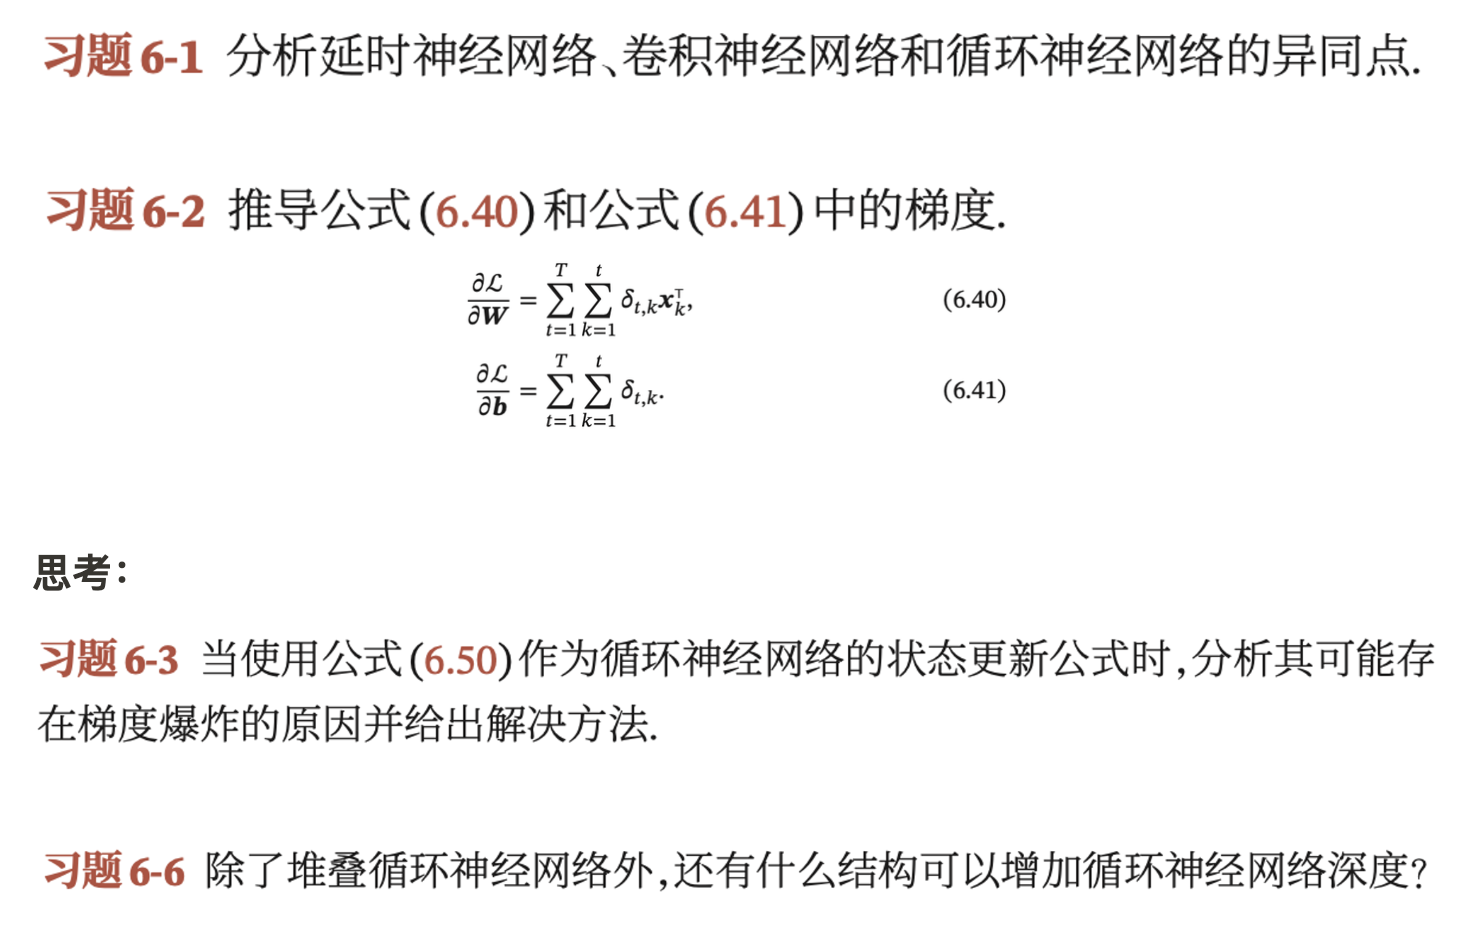
\includegraphics[width=1\linewidth]{第六章课后习题}
	\caption{第六章课后习题}
	\label{fig:}
\end{figure}

\subsection{习题6-1}
延时神经网络(FNN)是基本的前馈型神经网络,适用于静态输入-输出映射问题,但不具备处理序列数据的能力。

卷积神经网络(CNN)主要处理网格状数据,如图像,通过卷积和池化提取局部特征,适用于静态输入-输出映射问题,例如图像分类和目标检测。

循环神经网络(RNN)具有循环连接,能够处理序列数据,适用于时序数据和需要考虑上下文关系的任务,但容易受梯度消失和梯度爆炸问题的影响。

共同点包括属于深度学习范畴、使用反向传播算法训练、可通过堆叠多个层增加深度。不同之处在于网络结构、适用场景、记忆能力和参数共享。

\subsection{习题6-2}
为了推导公式(6.40)和(6.41)中的梯度,我们首先需要了解一些符号的含义。在这里,我们使用了以下符号:

\( \mathcal{L} \) 是损失函数。
\( \boldsymbol{W} \) 是权重矩阵。
\( \boldsymbol{b} \) 是偏置向量。
\( T \) 是序列的长度。
\( \delta_{t, k} \) 是一个指示函数,如果 \( t = k \) 则为1,否则为0。
\( \boldsymbol{x}_{k\cdot} \) 是输入序列在时间步 \( k \) 处的特征向量。
\( \boldsymbol{h}_t \) 是时刻 \( t \) 处的隐状态。
\( k^* \) 是目标时刻。

现在我们来推导这两个梯度:

1. 推导 \( \frac{\partial \mathcal{L}}{\partial \boldsymbol{W}} \):

我们有损失函数 \( \mathcal{L} \) 关于权重矩阵 \( \boldsymbol{W} \) 的梯度为:

\[ \frac{\partial \mathcal{L}}{\partial \boldsymbol{W}} = \sum_{t=1}^T \sum_{k=1}^t \delta_{t, k} \boldsymbol{x}_{k\cdot}^{\top} \]

这里,\( \delta_{t, k} \) 的存在保证了只有在 \( t = k \) 时才会有梯度,因此在每个时间步只有一个 \( \boldsymbol{x}_{k\cdot}^{\top} \) 被选择。

2. 推导 \( \frac{\partial \mathcal{L}}{\partial \boldsymbol{b}} \):

我们有损失函数 \( \mathcal{L} \) 关于偏置向量 \( \boldsymbol{b} \) 的梯度为:

\[ \frac{\partial \mathcal{L}}{\partial \boldsymbol{b}} = \sum_{i=1}^T \sum_{k=1}^t \delta_{t, k^* \cdot} \]

其中 \( k^* \) 是目标时刻,该梯度的存在保证了只有在 \( t = k^* \) 时才会有梯度。

\subsection{习题6-3}
在循环神经网络(RNN)中,如果使用状态更新公式 \( \boldsymbol{h}_t = \boldsymbol{h}_{t-1} + g(\boldsymbol{x}_t, \boldsymbol{h}_{t-1}; \boldsymbol{\theta}) \),其中 \( g \) 是一个包含可学习参数 \(\boldsymbol{\theta}\) 的函数,可能会导致梯度爆炸的问题。梯度爆炸指的是在反向传播过程中,梯度的绝对值变得非常大,导致权重的更新过大,使网络的权重无法稳定地收敛。

梯度爆炸的原因主要是由于循环连接导致梯度在时间步上累积。如果 \( g \) 的梯度较大,多次连续相乘(时间步数较大)会导致梯度指数级增长,从而引发梯度爆炸的问题。

解决梯度爆炸问题的方法包括:梯度裁剪、权重正则化、使用合适的激活函数等。
\subsection{习题6-6}
当增加循环神经网络(RNN)的深度时,除了使用堆叠循环神经网络外,还有其他方法:

1. 改进型结构(GRU和LSTM):GRU和LSTM解决了传统RNN中的梯度问题,通过引入门控机制,提高网络在深度方向上的训练效果。

2.双向RNN:同时处理正向和反向信息,更全面地捕捉上下文信息。

3. 残差连接:类似于ResNet,引入残差连接有助于更好地传播梯度,训练更深层次的网络。

4. 金字塔式RNN:通过下采样减小时间步,减轻梯度传播难度,允许更深层次的学习。

5. 分层RNN:
引入多层次结构,使网络能够学习和表示多个时间尺度的信息。


\section{第七章课后习题}
习题7-1 在小批量梯度下降中,试分析为什么学习率要和批量大小成正比.

习题 7-6 参见公式(7.51). 在批量归一化中,以 𝑓(⋅) 取 Logistic 函数或 ReLU 函数为例,分析以下两种归一化方法的差异:𝑓(BN(𝑾𝒂(𝑙−1) + 𝒃))和𝑓(𝑾BN(𝒂(𝑙−1)) + 𝒃).

习题7-10 试分析为什么不能在循环神经网络中的循环连接上直接应用丢弃法?
\subsection{习题7-1}在小批量梯度下降中,每次更新模型参数时使用从整个训练集中随机抽取的小批量数据。学习率与批量大小的正比关系有以下优势:

1. 减少噪音影响:采用随机子集数据进行参数更新,学习率与批量大小成正比有助于减小随机性(噪音)对梯度更新的影响,提高稳定性。

2. 提高计算效率:使用小批量数据计算梯度可显著提高效率,学习率与批量大小成正比有助于保持相对较大的梯度更新,减小时间成本。

3. 适应性学习率:自适应学习率算法可根据参数的历史梯度信息调整学习率,学习率与批量大小的正比关系更为合理。

4. 避免更新波动:学习率与批量大小成正比可一定程度上避免梯度更新引起的波动,使训练更加稳定。

\subsection{习题7-6}
在批量归一化中,有两种常见的归一化方法:在激活函数之前(\(f(BN(Wa^{(l-1)} + b))\))和在激活函数之后(\(f(W \cdot BN(a^{(l-1)}) + b)\))。考虑 Logistic 函数和 ReLU 函数。

1. 在激活函数之前进行批量归一化:在 Batch Normalization 之前使用 ReLU 可能导致部分输入在 Batch Normalization 后仍为零,因为 ReLU 可能将一些负值归零,影响 Batch Normalization 效果。

2. 在激活函数之后进行批量归一化:在 Batch Normalization 之后使用 ReLU,确保 Batch Normalization 不会将激活函数中的零值归一化为非零。

\subsection{习题7-10}
在循环神经网络(RNN)中,直接应用丢弃法(Dropout)在循环连接上存在问题。丢弃法是一种用于防止过拟合的技术,通过在训练时随机将一部分神经元的输出置零来减少神经元之间的依赖性。然而,在RNN的循环连接上使用丢弃法涉及到时间序列的传播,导致以下问题:

1. 时序依赖性:RNN的循环连接涉及对时间序列的处理,隐藏状态在每个时间步依赖于前一个时间步。应用丢弃法可能破坏隐藏状态的时序依赖性,导致在处理时序数据时出现问题。

2. 梯度传播问题:丢弃法引入的随机失活可能导致梯度的不稳定传播,在循环连接上更为显著,因为丢弃的神经元在每个时间步都可能不同,难以稳定梯度传播,导致训练不稳定。

3. 参数共享问题:循环神经网络中参数是共享的,即相同的权重在不同时间步上使用。应用丢弃法可能破坏参数共享,使网络学习到的模式不够稳定。
\end{document}
